\documentclass[12pt]{article}
\usepackage[margin=2.5cm]{geometry}
\usepackage{enumerate}
\usepackage{amsfonts}
\usepackage{amsmath}
\usepackage{fancyhdr}
\usepackage{amsmath}
\usepackage{amssymb}
\usepackage{amsthm}
\usepackage{mdframed}
\usepackage{graphicx}
\usepackage{subcaption}
\usepackage{adjustbox}
\usepackage{listings}
\usepackage{xcolor}
\usepackage{booktabs}
\usepackage[utf]{kotex}
\usepackage{hyperref}

\definecolor{codegreen}{rgb}{0,0.6,0}
\definecolor{codegray}{rgb}{0.5,0.5,0.5}
\definecolor{codepurple}{rgb}{0.58,0,0.82}
\definecolor{backcolour}{rgb}{0.95,0.95,0.92}

\lstdefinestyle{mystyle}{
    backgroundcolor=\color{backcolour},
    commentstyle=\color{codegreen},
    keywordstyle=\color{magenta},
    numberstyle=\tiny\color{codegray},
    stringstyle=\color{codepurple},
    basicstyle=\ttfamily\footnotesize,
    breakatwhitespace=false,
    breaklines=true,
    captionpos=b,
    keepspaces=true,
    numbers=left,
    numbersep=5pt,
    showspaces=false,
    showstringspaces=false,
    showtabs=false,
    tabsize=1
}

\lstset{style=mystyle}

\pagestyle{fancy}
\renewcommand{\headrulewidth}{0.4pt}
\lhead{CSC 209}
\rhead{Review 8 Solution}

\begin{document}
\title{CSC 209 Review 8 Solution}
\maketitle

\bigskip

\begin{enumerate}[1.]
    \item

    I need to create a wrapper function \texttt{my\_malloc} that does the following:

    \bigskip

    \begin{itemize}
        \item ask \texttt{my\_malloc} it to allocate \texttt{n} bytes
        \item call \texttt{malloc}
        \item test \texttt{malloc} doesn't have a null pointer
        \item return pointer from \texttt{malloc}
    \end{itemize}

    \bigskip

    The solution to this problem is:

\begin{lstlisting}[language=c]
    void *my_malloc(int n) {
        void *p;

        p = malloc(n);

        if (!p) {
            printf("ERROR: Malloc allocation failed");
        }

        return p;
    }
\end{lstlisting}

    \underline{\textbf{Notes}}

    \begin{itemize}
        \item Learned that void function can return value
        \item \textbf{Dynamic Storage Allocation}

        \begin{itemize}
            \item Allows to allocate storage during program execution
            \item Allows to create data structures and shink and grow array as needed
            \item e.g. \texttt{malloc}, \texttt{calloc}, \texttt{realloc}
        \end{itemize}
        \item \textbf{Memory Allocation Functions}

        \begin{itemize}
            \item \texttt{malloc} - Allocates a block of memory but doesn't initialize it

            \begin{itemize}
                \item doesn't initialize the allocated memory
                \item more efficient than \texttt{calloc}
                \item accessing the content $\to$ segmentation fault (accessing value at invalid mem. location)
                or garbage values
            \end{itemize}

            \item \texttt{calloc} - Allocates a block of memory and clears it

            \begin{itemize}
                \item allocates memory and \underline{initializes the memory block} to zero
                \item accessing the content of blocks would return 0
            \end{itemize}

            \item \texttt{realloc} - Resizes a previously allocated block of memory
        \end{itemize}

        \item \textbf{Null Pointer}

        \begin{itemize}
            \item is returned when it fails to allocate a block of memory large
            enough to satisfy the request
        \end{itemize}

        \bigskip

        \underline{\textbf{Example}}

        \begin{center}
        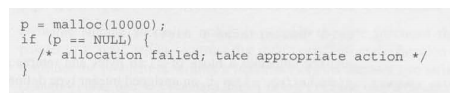
\includegraphics[width=\linewidth]{images/review_8_solution_1.png}
        \end{center}
    \end{itemize}

    \item

    I need to write a function named \texttt{duplicate} that uses dynamic storage
    allocation to create a copy of a string.

    \bigskip

    The requirements of the function are

    \begin{itemize}
        \item \texttt{duplicate} allocates space for a string of the same length as \texttt{str}
        \item \texttt{duplicate} copies the contents of str into the new string
        \item \texttt{duplicate} returns a pointer to it
        \item \texttt{duplicate} returns a null pointer if the memory allocation fails
    \end{itemize}

    \bigskip

    The solution to this problem is:

    \bigskip

\begin{lstlisting}[language=c]
    #include <stdio.h>
    #include <stdlib.h>  // malloc
    #include <string.h>  // strlen

    char *duplicate(const char *str);

    int main(void) {
        char s[] = "hello world", *p;

        p = duplicate (s);

        printf("Duplicate: %s\n", p);

        free(p);
        return 0;
    }


    char *duplicate(const char *str) {
        char *p, *q;
        const char *r;

        int n = strlen(str);

        p = (char *)malloc(n + 1);

        if (!p) {
            return p;
        }

        r = str;
        q = p;
        while (r < str + n) {
            *q = *r;
            q++;
            r++;
        }

        *q = '\0';

        return p;
    }
\end{lstlisting}

    \bigskip

    \begin{mdframed}
    \underline{\textbf{Correct Solution:}}

\begin{lstlisting}[language=c]
    #include <stdio.h>
    #include <stdlib.h>  // malloc
    #include <string.h>  // strlen

    char *duplicate(const char *str);

    int main(void) {
        char s[] = "hello world", *p, *q;
        ;
        p = duplicate (s);

        printf("Duplicate: %s\n", p);

        free(p);
        return 0;
    }


    char *duplicate(const char *str) {
        char *p, *q;
        const char *r;

        int n = strlen(str);

        p = (char *)malloc(n + 1);

        if (!p) {
            p = ((void*)0);
            return p;
        }

        r = str;
        q = p;
        while (r < str + n) {
            *q = *r;
            q++;
            r++;
        }

        *q = '\0';

        return p;
    }
\end{lstlisting}

    \end{mdframed}

    \underline{\textbf{Note}}

    \begin{itemize}
        \item Null pointer has value \texttt{((void*)0)}
        \item \texttt{const} tag in parameter prevetns the function from modifying
        what it's pointer variable is pointing to.

        \begin{itemize}
            \item value is modifiable
            \item changes the parameter to pass by value
        \end{itemize}
    \end{itemize}

    \item

\begin{lstlisting}[language=c]
    int *create_array(int n, int initial_value) {
        int *array;

        array = malloc(n * sizeof(int));

        if (array == NULL) {
            return array;
        }

        for(int i = 0; i < n; i++){
            array[i] = initial_value;
        }

        return array
    }
\end{lstlisting}


    \bigskip

    \underline{\textbf{Notes}}

    \begin{itemize}
        \item \textbf{Dynamically Allocated Arrays}
        \begin{itemize}
            \item \textbf{Syntax:}

            \bigskip

            \texttt{int *a;}

            \texttt{a = malloc(n * sizeof(int));}

            \bigskip
            \item returns null pointer if allocation fails
        \end{itemize}
    \end{itemize}

    \item

    \bigskip

\begin{lstlisting}[language=c]
    #include <stdio.h>
    #include <stdlib.h>
    #include <string.h>

    struct point {int x, y;};
    struct rectangle {struct point upper_left, lower_right;};

    int main(void) {

        struct rectangle *p;

        p = malloc(sizeof(struct rectangle));

        p->upper_left.x = 10;
        p->upper_left.y = 25;
        p->lower_right.x = 20;
        p->lower_right.y = 15;

        printf("%d %d %d %d",
            p->upper_left.x,
            p->upper_left.y,
            p->lower_right.x,
            p->lower_right.y
        );

        return 0;
    }
\end{lstlisting}

    \underline{\textbf{Notes}}

    \begin{itemize}
        \item -$>$ doesn't carry over to accessing nested members. Only works when
        struct is a pointer

        \bigskip

        \underline{\textbf{Example}}

        \bigskip

        \texttt{p-$>$upper\_left.x}

        \bigskip
        \item \textbf{Linked Lists}

        \begin{itemize}
            \item \textbf{Declaring Node Type}

            \begin{itemize}
                \item \textbf{Syntax (Node structure):}

                \begin{center}
                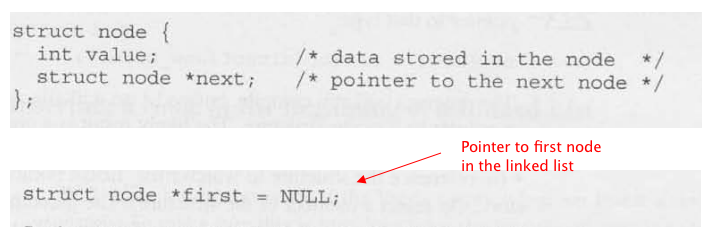
\includegraphics[width=\linewidth]{images/review_8_solution_2.png}
                \end{center}

            \end{itemize}

            \item \textbf{Creating a Node}

            \begin{itemize}
                \item \textbf{Syntax (Allocating using malloc):}

                \bigskip

                \texttt{struct node *new\_node;}

                \texttt{new\_node = malloc(sizeof(struct node));}

                \bigskip

                \item Assigning value

                \bigskip

                \texttt{(*new\_node).value = 10;}

                \bigskip

            \end{itemize}
            \item \textbf{-$>$ Operator}

            \begin{itemize}
                \item is a short form of \texttt{(*STRUCT\_NAME).MEMBER\_NAME}

                \bigskip

                \underline{\textbf{Example}}

                \bigskip

                \texttt{(*new\_node).value = 10;}

                \bigskip

                Is the same as

                \bigskip

                \texttt{new\_node-$>$value = 10;}
            \end{itemize}
        \end{itemize}
    \end{itemize}

    \item

    \texttt{b)} and \texttt{c)} are legal

    \bigskip

    \item

\begin{lstlisting}[language=c]
    struct node *delete_from_list(struct node *list, int n)
    {
        struct node *curr, *to_be_freed;

        for (curr = list; curr != NULL && curr->value != n; curr = curr->next) {
            if (curr->next != NULL && curr->next->value == n) {
                to_be_freed = curr->next;
                curr->next = curr->next->next;
                free(to_be_freed);

                return list;
            }
        }


        return list;

    }
\end{lstlisting}

    \bigskip

    \underline{\textbf{Notes}}

    \begin{itemize}
        \item \textbf{Searching a Linked List}

        \begin{itemize}
            \item \textbf{Syntax:} \texttt{for (p = first; p != NULL; p = p -$>$next)}

            \bigskip

            \underline{\textbf{Example:}}

            \bigskip

            \begin{center}
            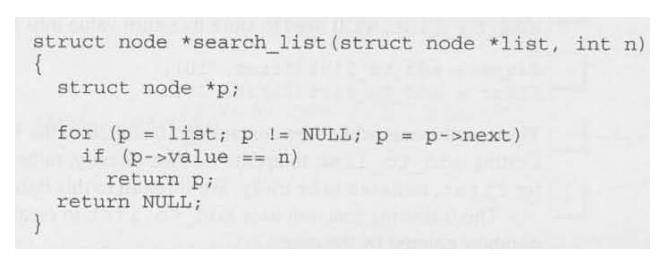
\includegraphics[width=0.9\linewidth]{images/review_8_solution_3.png}
            \end{center}
        \end{itemize}
        \item \textbf{Deleting Node from a List}

        \begin{itemize}
            \item Steps

            \begin{enumerate}[1.]
                \item Locate the node to be deleted

                \begin{itemize}
                    \item \textbf{Syntax (Searching for the node of value \texttt{n} to be deleted):}

                    \bigskip

                    \begin{center}
                    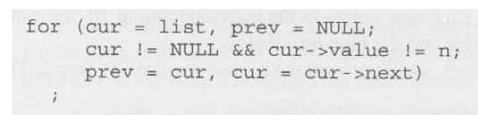
\includegraphics[width=0.8\linewidth]{images/review_8_solution_4.png}
                    \end{center}
                \end{itemize}

                \item Alter the previous node so that it "bypasses" the deleted node

                \begin{center}
                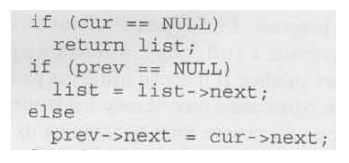
\includegraphics[width=0.6\linewidth]{images/review_8_solution_5.png}
                \end{center}

                \item Call \texttt{free} to reclaim the space occupied by the deleted code

                \begin{center}
                
\includegraphics[width=0.6\linewidth]{images/review_8_solution_6.png}
                \end{center}
            \end{enumerate}

            \bigskip

            Putting together, we have

            \begin{center}
            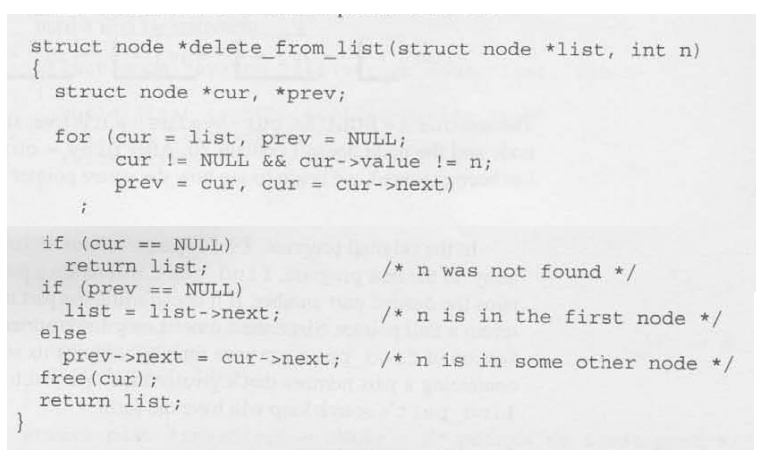
\includegraphics[width=\linewidth]{images/review_8_solution_7.png}
            \end{center}
        \end{itemize}
    \end{itemize}

    \item

    The statement is incorrect because it removes the current node before its
    pointer moves to the next node.

    \bigskip

    As a result, the remaining nodes cannot be removed, and this is not good.

    \bigskip

    To fix the problem, the pointer \texttt{p} must move to the next before removing
    the current node, as shown below:


\begin{lstlisting}[language=c]
    struct node *to_be_freed;

    for (p = first; p != NULL;) {
        to_be_freed = p;
        p = p->next;
        free(p);
    }
\end{lstlisting}

    \item

\begin{lstlisting}[language=c]
    #include <stdio.h>
    #include <stdbool.h>
    #include <stdlib.h>
    #include <stddef.h> // NULL

    struct node {
        int value;
        struct node *next;
    };

    struct node *top = NULL;

    void make_empty(struct node *top) {
        struct node *temp;

        while (top != NULL) {
            temp = top;
            top = top->next;
            free(temp);
        }
    }

    bool is_empty(void) {
        if (top == NULL) {
            return true;
        }

        return false;
    }

    bool push (int n, struct node *top) {
        struct node *new_node;

        new_node = malloc(sizeof(struct node));

        if (new_node == NULL) {
            return false;
        }

        new_node->value = n;

        if (top == NULL) {
            top = new_node;
        } else {
            new_node->next = top->next;
            top->next = new_node;
        }

        return true;
    }

    int pop(void) {
        struct node *temp;
        int return_val;

        temp = top;
        return_val = temp->value;
        top = top->next;
        free(temp);

        return return_val;
    }
\end{lstlisting}

    \item

    True. With \& sign, the \texttt{struct node} becomes \texttt{type pointer}.

    \bigskip

    With pointer, \texttt{-$>$} can be used.

    \bigskip

    Thus, \texttt{x.a} is the same as \texttt{(\&x)-$>$a}.

    \item

\begin{lstlisting}[language=c]
    struct part {
        int number;
        char name[NAME_LEN+1];
        int on_hand;
    };

    ...

    void print_part(struct part *p)
    {
        printf("Part number: %d\n", p->number);
        printf("Part name: %s\n", p->name);
        printf("quantity on hand: %d\n", p->on_hand);
    }
\end{lstlisting}

    \item

\begin{lstlisting}[language=c]
    #include <stddef.h>

    struct node {
        int value;
        struct node *next;
    };

    int count_occurences (struct node *list, int n)
    {
        int count;
        struct node *top;

        for (top=list; top != NULL; top = top->next) {
            if (top->value == n) {
                count++;
            }
        }

        return count;
    }
\end{lstlisting}


    \item

\begin{lstlisting}[language=c]
    #include <stddef.h>

    struct node {
        int value;
        struct node *next;
    };

    struct node *find_last (struct node *list, int n)
    {
        struct node *last = NULL, *top;

        for (top=list; top != NULL; top = top->next) {
            if (top->value == n) {
                last = top;
            }
        }

        return last;
    }
\end{lstlisting}

    \item

\begin{lstlisting}[language=c]
    #include <stdio.h>
    #include <stdbool.h>
    #include <stdlib.h>
    #include <stddef.h>

    struct node {
        int value;
        struct node *next;
    };
    struct node *insert_into_ordered_list (struct node *list, struct node *new_node);

    struct node *insert_into_ordered_list (struct node *list,
                                          struct node *new_node)
    {
        struct node *cur, *prev;

        for (cur = list, prev = NULL;
             cur != NULL && cur->value < new_node->value;
             prev=cur, cur = cur->next)
             ;

        prev->next = new_node;
        new_node->next = cur;
        return list;
    }

\end{lstlisting}

    \bigskip

    \underline{\textbf{Notes}}

    \begin{itemize}
        \item Passing \texttt{NULL} results in segmentation fault

        \bigskip

        \texttt{insert\_ordered\_list(NULL, 4);}
    \end{itemize}

    \item

\begin{lstlisting}[language=c]
    void delete_from_list(struct node **list, int n)
    {
        struct node *cur, *prev = NULL;
        cur = *list;

        while (cur != NULL) {
            if (cur->value == n) {
                break;
            }

            prev = cur;
            cur = cur->next;

        }


        if (prev == NULL) {
            *list = (*list)->next;
        } else {
            prev->next = cur->next;
        }

        free(cur);
    }
\end{lstlisting}

    \bigskip

    \underline{\textbf{Notes}}

    \begin{itemize}
        \item \textbf{Pointers to Pointers}

        \begin{itemize}
            \item \textbf{Syntax:} \texttt{TYPE **ptr}
            \item pops up frequently in data structures
            \item is used to store the address of the first pointer

            \begin{center}
            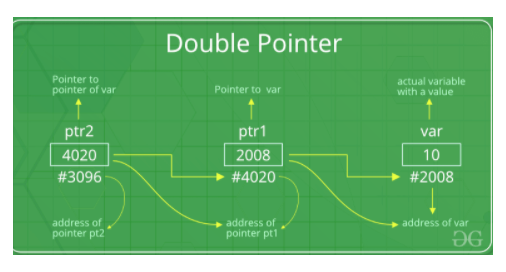
\includegraphics[width=\linewidth]{images/review_8_solution_8.png}
            \end{center}

            \bigskip

            \underline{\textbf{Example}}

            \bigskip

            Passing a pointer \texttt{*first} that points to \texttt{malloc(struct node)} (a pointer pointing to malloc)
            to function \texttt{*add\_to\_list(struct node *list, int n)} (nono).

            \bigskip

            \begin{itemize}
                \item at point of call, \texttt{first} is copied to \texttt{list}
                \item \texttt{*list} is a pointer that must point to \texttt{*first}. So, this is invalid form.
                For above to be valid, double pointer must be used.

                \bigskip

                \texttt{*add\_to\_list(struct node **list, int n)}
            \end{itemize}

            \item \texttt{**list} refers to value in \texttt{malloc(struct node)}
            \item \texttt{*list} refers to the address of variable (\texttt{first}) that points to \texttt{malloc(struct node)}
            \item \texttt{\&list} refers to address of variable list
        \end{itemize}
    \end{itemize}

    \item

    \bigskip

    \underline{\textbf{Notes:}}

    \begin{itemize}
        \item \textbf{Pointer to Functions}

        \begin{itemize}
            \item \textbf{Function Pointers to Arguments}

            \bigskip

            \underline{\textbf{Example}}

            \bigskip

            \begin{center}
            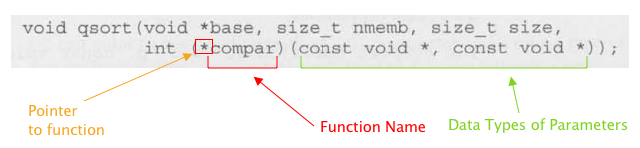
\includegraphics[width=\linewidth]{images/review_8_solution_9.png}
            \end{center}

            \begin{itemize}
                \item The passed function can be used as follows

                \bigskip

                \texttt{y = (*f)(x)}
            \end{itemize}

        \end{itemize}
    \end{itemize}

\end{enumerate}

\end{document}